% Generated by scripts/make_explanation_figures.py from experiment_0013 (do not edit by hand).
% Model: COVER
\documentclass[tikz,border=3pt]{standalone}
\usepackage[T1]{fontenc}
\usepackage[utf8]{inputenc}
\usepackage{newtxtext,newtxmath}
\usetikzlibrary{positioning,arrows.meta,calc}

\definecolor{neural}{HTML}{2F6DB5}
\definecolor{neuralbg}{HTML}{E8F0FA}
\definecolor{logic}{HTML}{2E8B57}
\definecolor{logicbg}{HTML}{E6F4EC}
\definecolor{relneg}{HTML}{C0392B}

\tikzset{
  tok/.style={draw=neural!80, fill=white, rounded corners=1.5pt, inner sep=1.6pt, font=\scriptsize,
              minimum height=4mm, anchor=base},
  htok/.style={tok, fill=neural!12},
  stok/.style={tok, draw=black!25, text=black!45},
  aedge/.style={line width=#1, draw=logic},
  cedge/.style={line width=#1, draw=relneg},
  ledge/.style={line width=#1, draw=neural, densely dashed},
  rlab/.style={font=\tiny, fill=white, inner sep=0.6pt},
}
\newcommand{\bars}[4]{%
  \fill[logic]  (#1-0.17,0.05) rectangle ++(0.15,{0.8*#2});
  \fill[relneg] (#1+0.02,0.05) rectangle ++(0.15,{0.8*#3});
  \node[font=\tiny, anchor=north] at (#1-0.095,0.03) {$s$};
  \node[font=\tiny, anchor=north] at (#1+0.095,0.03) {$c$};
  \node[font=\tiny, anchor=north] at (#1,-0.22) {$#2\,/\,#3$};
  \node[font=\tiny, anchor=north, text=black!60] at (#1,-0.47) {$\omega{=}#4$};
}
\newcommand{\sbar}[3]{%
  \fill[logic]  (#1-0.075,0.05) rectangle ++(0.15,{0.8*#2});
  \node[font=\tiny, anchor=north] at (#1,0.03) {$s$};
  \node[font=\tiny, anchor=north] at (#1,-0.22) {$#2$};
  \node[font=\tiny, anchor=north, text=black!60] at (#1,-0.47) {$\omega{=}#3$};
}
\providecommand{\Pcov}{P_{\mathrm{cov}}}
\providecommand{\Pnc}{P_{\neg\mathrm{conf}}}
\providecommand{\E}{\textsc{e}}
\providecommand{\N}{\textsc{n}}
\providecommand{\C}{\textsc{c}}

\begin{document}
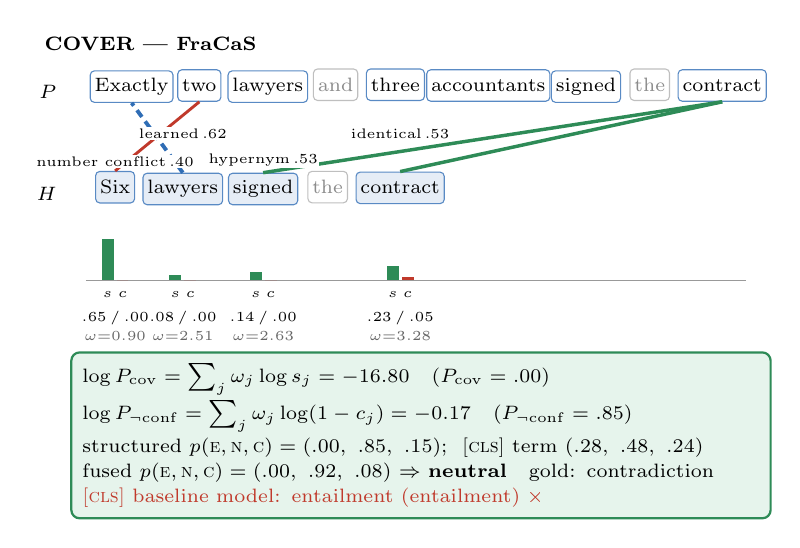
\begin{tikzpicture}
\begin{scope}[xshift=0.00cm]
\node[font=\scriptsize\itshape, anchor=east] at (-0.35,2.45) {$P$};
\node[font=\scriptsize\itshape, anchor=east] at (-0.35,1.15) {$H$};
\node[tok] (p1) at (0.48,2.45) {Exactly};
\node[tok] (p2) at (1.34,2.45) {two};
\node[tok] (p3) at (2.21,2.45) {lawyers};
\node[stok] (pw3) at (3.07,2.45) {and};
\node[tok] (p5) at (3.83,2.45) {three};
\node[tok] (p6) at (5.01,2.45) {accountants};
\node[tok] (p8) at (6.25,2.45) {signed};
\node[stok] (pw7) at (7.06,2.45) {the};
\node[tok] (p10) at (7.98,2.45) {contract};
\node[htok] (h14) at (0.27,1.15) {Six};
\node[htok] (h15) at (1.13,1.15) {lawyers};
\node[htok] (h16) at (2.15,1.15) {signed};
\node[stok] (hw3) at (2.97,1.15) {the};
\node[htok] (h18) at (3.89,1.15) {contract};
\draw[cedge=1.04pt] (h14.north) -- (p2.south);
\draw[ledge=1.39pt] (h15.north) -- (p1.south);
\draw[aedge=1.25pt] (h16.north) -- (p10.south);
\draw[aedge=1.25pt] (h18.north) -- (p10.south);
\node[rlab, anchor=south] at (0.27,1.47) {number conflict\,.40};
\node[rlab, anchor=south] at (1.13,1.83) {learned\,.62};
\node[rlab, anchor=south] at (2.15,1.47) {hypernym\,.53};
\node[rlab, anchor=south] at (3.89,1.83) {identical\,.53};
\draw[black!40] (-0.1,0.05) -- (8.28,0.05);
\bars{0.27}{.65}{.00}{0.90}
\bars{1.13}{.08}{.00}{2.51}
\bars{2.15}{.14}{.00}{2.63}
\bars{3.89}{.23}{.05}{3.28}
\end{scope}
\node[draw=logic, fill=logicbg, rounded corners=3pt, line width=0.8pt, font=\scriptsize, align=left, anchor=north west, text width=8.60cm, inner sep=4pt] (agg) at (-0.3,-0.85) {%
  $\log\Pcov=\sum_j\omega_j\log s_j=-16.80$\quad($\Pcov=.00$)\\[1pt]$\log\Pnc=\sum_j\omega_j\log(1-c_j)=-0.17$\quad($\Pnc=.85$)\\[1pt]structured $p(\E,\N,\C)=(.00,\ .85,\ .15)$;\ \ \textsc{[cls]} term $(.28,\ .48,\ .24)$\\[1pt]fused $p(\E,\N,\C)=(.00,\ .92,\ .08)$ $\Rightarrow$ \textbf{neutral}\quad gold: contradiction\\[1pt]\textcolor{relneg}{\textsc{[cls]} baseline model: entailment (entailment) \texttimes}};
\node[font=\scriptsize\bfseries, anchor=south west] at (-0.75,2.85) {COVER --- FraCaS};
\end{tikzpicture}
\end{document}
